\documentclass[11pt]{beamer}
\usetheme{CambridgeUS}
\usepackage[utf8]{inputenc}
\usepackage{amsmath}
\usepackage{amsfonts}
\usepackage{amssymb}
\usepackage{graphicx}
\usepackage{pgfpages}
\usepackage{framed}
\usepackage{xcolor}
\usepackage[most]{tcolorbox}
\usepackage{soul}
\usepackage{empheq}

\newcommand*{\itemimg}[1]{%
  \raisebox{-.3\baselineskip}{%
    \includegraphics[
      height=\baselineskip,
      width=\baselineskip,
      keepaspectratio,
    ]{#1}%
  }%
}

\newtcbox{\mymath}[1][]{%
    nobeforeafter, math upper, tcbox raise base,
    enhanced, colframe=blue!30!black,
    colback=blue!10, boxrule=1pt,
    #1}

\newcommand{\highlight}[1]{%
  \colorbox{yellow!100}{$\displaystyle#1$}}

\author{Giovanni Della Lunga\\{\footnotesize giovanni.dellalunga@unibo.it}}
%\title{1.1 - Introduction to Machine Learning}
%\title{1.2 - Data Gathering with Pandas}
\title{2.1 - Training, Validation and Testing}
%\title{4.1 - Linear and Logistic Regression}
%\title{4.2 - Decision Trees}
%\title{6 - Text Vectorization}
%\title{7 - Classification for Text Analysis}
%\title{8 - Clustering for Text Similarity}
%\title{9 - Information Extraction}
\subtitle{} % (optional)
\setbeamercovered{transparent} 
\institute{Introduction to Machine Learning for Finance} 
\date{Bologna - February-March, 2025} 


\begin{document}

\begin{frame}
\titlepage
\end{frame}

\AtBeginSection[]
{
\begin{frame}<beamer>
  \frametitle{Outline}
  \tableofcontents[currentsection]
\end{frame}
}
\AtBeginSubsection{\frame{\subsectionpage}}


%===================================================================================================
%__________________________________________________________________________
%
\subsection[subsection]{Training, Validation and Testing}
%__________________________________________________________________________
%
\begin{frame}{Training, Validation and Testing}
	\begin{itemize}
		\item When data is used for forecasting there is a danger that the machine learning model \textbf{will work very well for training data, but will not generalize well to other data};
		\item An obvious point is that it is important that the data used in a machine learning model be representative of the situations to which the model is to be applied;
		\item It is also important to test a model \textbf{out-of-sample}, by this we mean that \ul{the model should be tested on data that is different from the sample data used to determine the parameters of the model};
		\item Data scientist refer to the sample data as the \textbf{training set} and the data used to determine the accuracy of the model as the \textbf{test set};
		\item Often a \textbf{validation set} is used as well as we explain later;
	\end{itemize}
\end{frame}
%..................................................................
\begin{frame}{Training, Validation and Testing}
\begin{itemize}
\item We will illustrate the use of a training set and the test data set with a very simple Example (Hull, Chapter 1);
\item We suppose that awe are interested in forecasting the salaries of people from their age;
\item This simple regression model is an example of supervised learning...
\end{itemize}
\end{frame}
%..................................................................
\begin{frame}{Training Set}{Training, Validation and Testing}
\textbf{Table 1}. Salary as a function of Age for a certain profession in a certain area)
	\begin{center}
	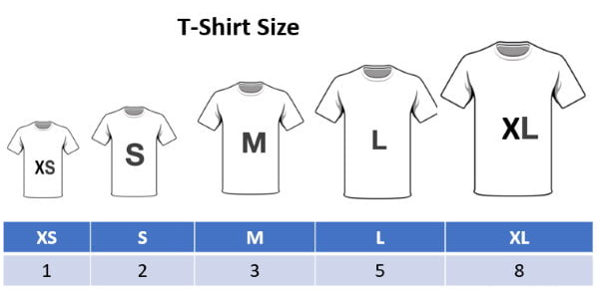
\includegraphics[scale=.6]{../05-pictures/lesson-2-2_pic_0.png}
	\end{center}
\end{frame}
%..................................................................
\begin{frame}{Training Set}{Training, Validation and Testing}
\textbf{Figure 1}. Scatter plot of Salary as a function of Age (see Table 1)
	\begin{center}
	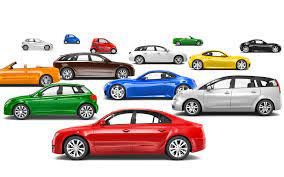
\includegraphics[scale=.6]{../05-pictures/lesson-2-2_pic_1.png}
	\end{center}
\end{frame}
%..................................................................
\begin{frame}{Training Set}{Training, Validation and Testing}
\textbf{Figure 2}. It's tempting to choose a model that fits the data really well for example with a polynomial of degree five (Y = Salary, X = Age):
	\begin{equation}
	Y = a + b_1X+b_2X^2+b_3X^3+b_4X^4+b_5X^5 \notag
	\end{equation}	 
	\begin{center}
	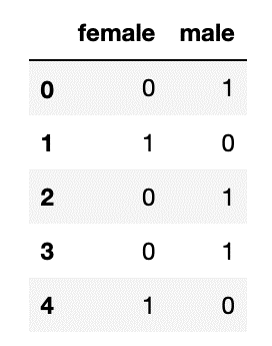
\includegraphics[scale=.6]{../05-pictures/lesson-2-2_pic_2.png}
	\end{center}
\end{frame}
%..................................................................
\begin{frame}{Discussion of Training Result}{Training, Validation and Testing}
\begin{itemize}
\item The model provides a good fit to the data;
\item The standard deviation of the difference between the salary given by the model and the actual salary for the ten individuals in the training data set (which is referred to as the \textbf{root mean square error (rmse)}) is \$12902;
\item However common sense would suggest that we many over-fitted the data;
\item We need to check the model out-of-sample;
\item To use the language of \textit{data science} we need to determine \ul{whether the model generalizes well to a new data set that is different from the training set}.
\end{itemize}
\end{frame}
%..................................................................
\begin{frame}{Validation Set}{Training, Validation and Testing}
\textbf {Figure 3}. An Out-of-Sample Validation Set
	\begin{center}
	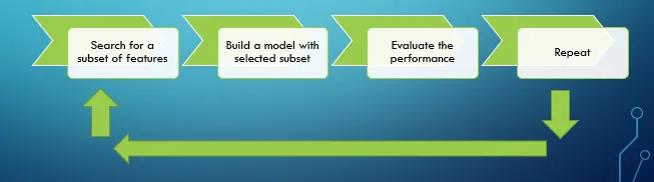
\includegraphics[scale=.6]{../05-pictures/lesson-2-2_pic_4.png}
	\end{center}
\end{frame}
%..................................................................
\begin{frame}{Validation and Testing: Validation Set}
\textbf{Figure 3}. Scatter Plot for Validation Set
	\begin{center}
	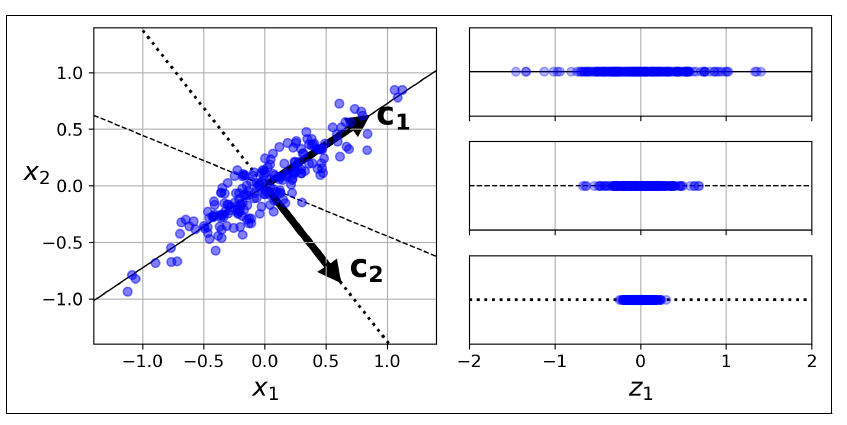
\includegraphics[scale=.5]{../05-pictures/lesson-2-2_pic_5.png}
	\end{center}
\end{frame}
%..................................................................
\begin{frame} {Validation and Testing: Discussion of Validation Result}
The Fifth Order Polynomial Model Does Not Generalize Well
	\begin{itemize}
		\item The root mean squared error (rmse) for the training      data set is \$12,902
		\item  The rmse for the test data set is \$38,794
		\item   We conclude that the model overfits the data
	\end{itemize}
	%\begin{center}
	%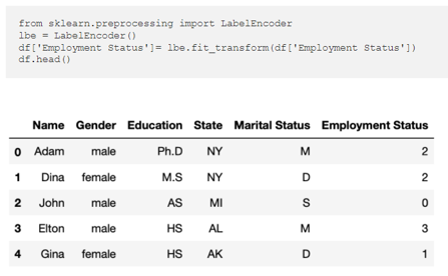
\includegraphics[scale=.5]{../05-pictures/lesson-2-2_pic_3.png}
	%\end{center}
\end{frame}
%..................................................................
\begin{frame}{Validation and Testing}

\textbf{Figure 4}. A Simpler Quadratic Model
	\begin{equation}
	Y = a + b_1X + b_2X^2 \notag
	\end{equation}		
	 
	\begin{center}
	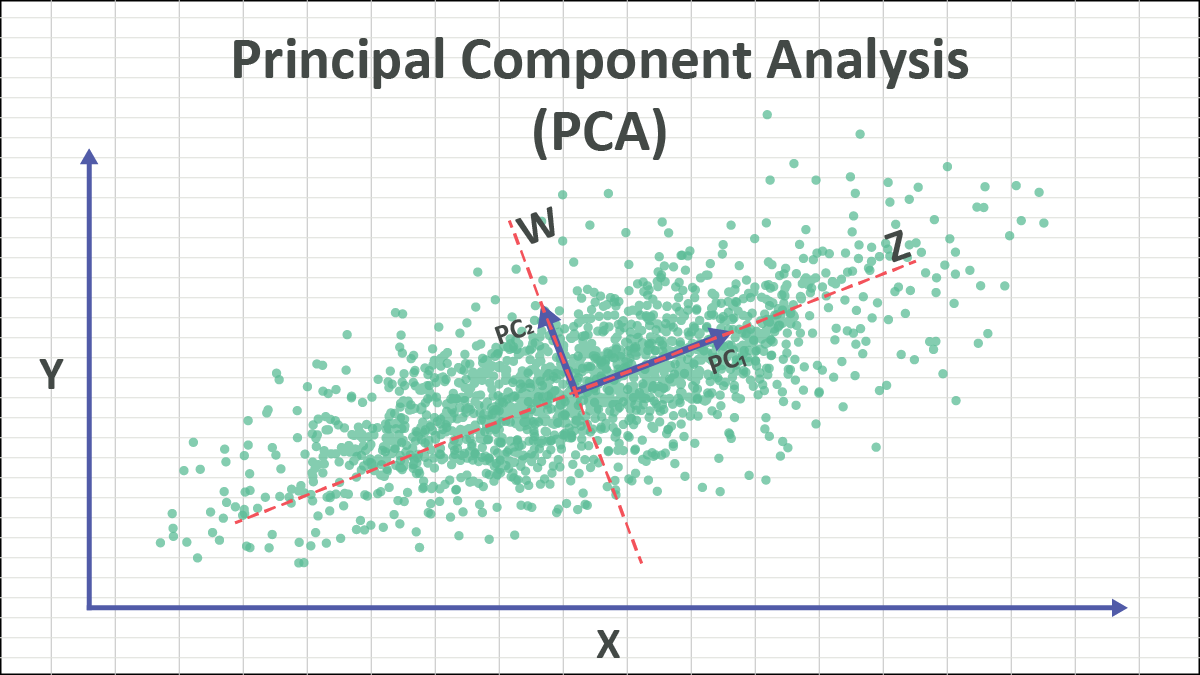
\includegraphics[scale=.6]{../05-pictures/lesson-2-2_pic_6.png}
	\end{center}
\end{frame}
%..................................................................
\begin{frame}{Validation and Testing}
\textbf{Figure 5 }. Linear Model
	\begin{equation}
		Y = a + b_1X \notag
	\end{equation}
	\begin{center}
	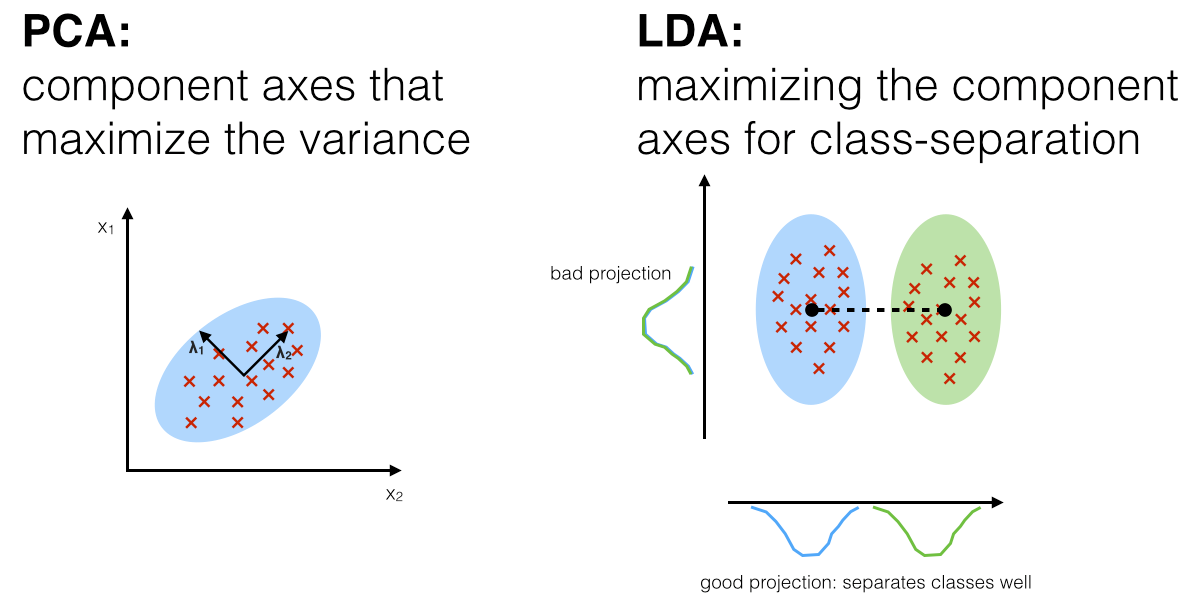
\includegraphics[scale=.6]{../05-pictures/lesson-2-2_pic_7.png}
	\end{center}
\end{frame}
%..................................................................
\begin{frame}{Validation and Testing}
\textbf{Table 3}. Summary of Results: The linear model under-fits while the 5th degree polynomial over-fits:
	\begin{center}
	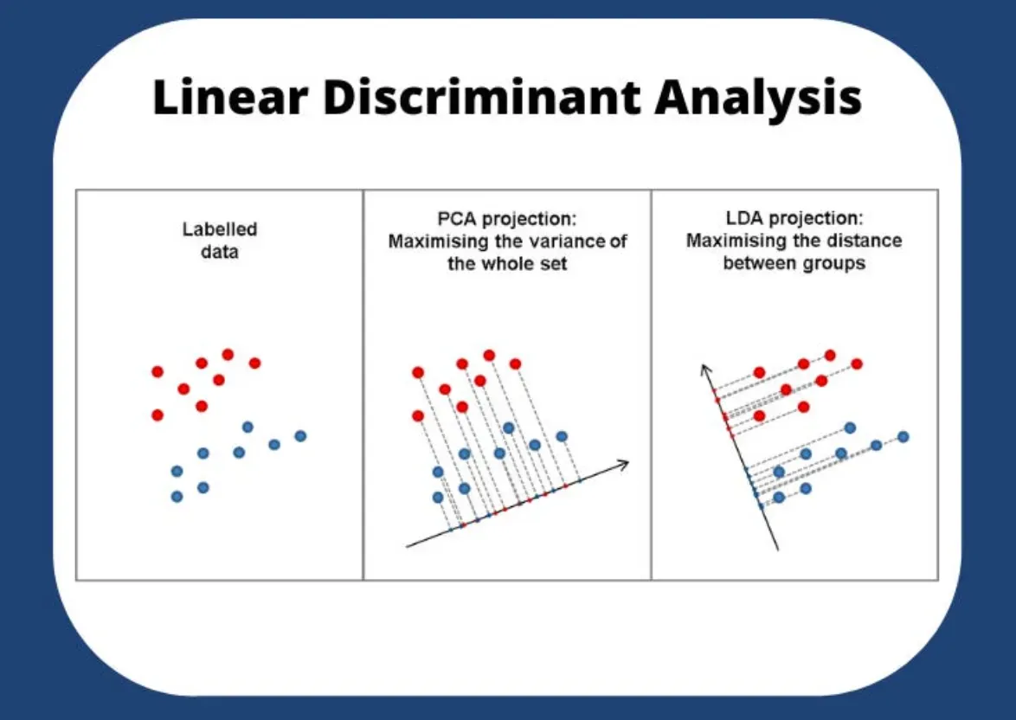
\includegraphics[scale=.6]{../05-pictures/lesson-2-2_pic_8.png}
	\end{center}
\end{frame}
%..................................................................
\begin{frame}{Validation and Testing}
\textbf{Table 3}. Summary of Results: The linear model under-fits while the 5th degree polynomial over-fits:
	\begin{center}
	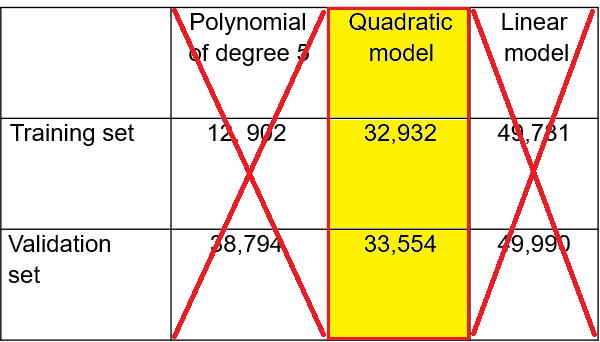
\includegraphics[scale=.6]{../05-pictures/lesson-2-2_pic_9.png}
	\end{center}
\end{frame}
%..................................................................
\begin{frame}{Validation and Testing}
\textbf{Figure 6}. Overfitting/Underfitting Example: predicting salaries for people in a certain profession in a certain area (only 10 observations)
	\begin{center}
	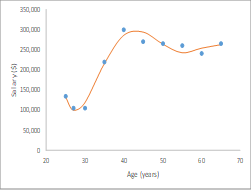
\includegraphics[scale=.5]{../05-pictures/lesson-2-2_pic_10.png}  \hfill
	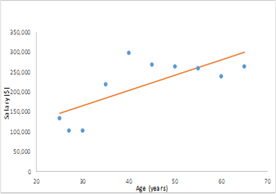
\includegraphics[scale=.5]{../05-pictures/lesson-2-2_pic_11.png}  \hfill
	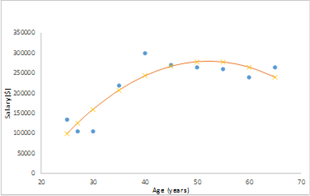
\includegraphics[scale=.5]{../05-pictures/lesson-2-2_pic_12.png}
	\end{center}
	Overfitting -------------- Underfitting	 ----------------- Best model?
\end{frame}
%..................................................................
\begin{frame}{Validation and Testing}
Typical Pattern of Errors for Training Set and Validation Set	
	\begin{center}
	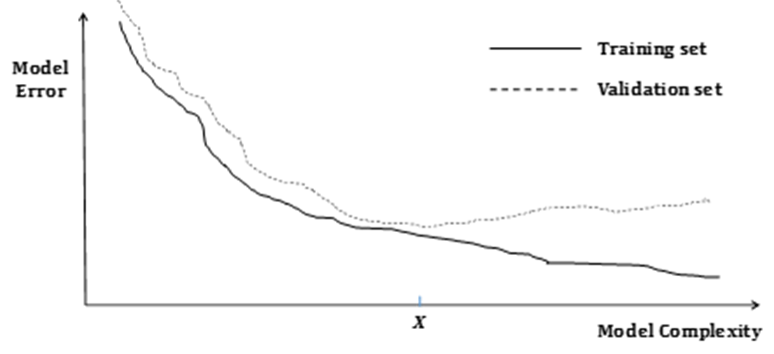
\includegraphics[scale=.6]{../05-pictures/lesson-2-2_pic_13.png}
	\end{center}
\end{frame}
%..................................................................
\begin{frame}{Validation and Testing}

ML Good Practice

	\begin{itemize}
		\item Divide data into three sets
		\item Training set
		\item Validation set
		\item Test set
		\item Develop different models using the \textbf{training set} and compare them using the \textbf{validation set};
		\item Rule of thumb: increase model complexity until model no longer generalizes well to the validation set;
		\item The \textbf{test set} is used to provide a final out-of-sample indication of how well the chosen model works;
	\end{itemize}
\end{frame}
%__________________________________________________________________________
%
\subsection[subsection]{Bias and Variance}
%__________________________________________________________________________
%
\begin{frame}{Bias and Variance}
\begin{itemize}
\item Suppose there is a relationship between an independent variable $x$ and a dependent variable $y$:

\begin{equation}
    y=f(x) + \epsilon
\end{equation}

where $\epsilon$ is an error term with mean zero and variance $\sigma^2$. 

\item The error term captures either genuine randomness in the data or noise due to measurement error.

\item Suppose we find, with a Machine Learning technique,  a deterministic model for this relationship:

\begin{equation}
    y = \hat f(x)
\end{equation}
 
\end{itemize}
\end{frame}
%..................................................................
\begin{frame}{Bias and Variance}
\begin{itemize}
\item Now it comes a new data point $x^\prime$ not in the training set and we want to predict the corresponding $y^\prime$;

\item The error we will observe in our model at point $x^\prime$ is going to be

\begin{equation}
    \hat f(x^\prime) - f(x^\prime) - \epsilon
\end{equation}

\item There are two different sources of error in this equation. 

\item The first one is included in the factor $\epsilon$; 

\item The second one, more interesting, is due to what is in our training set. 

\item A robust model should give us the same prediction whatever data we used for training out model.
\end{itemize}
\end{frame}
%..................................................................
\begin{frame}{Bias and Variance}
\begin{itemize}
\item Let's look at the average error:

\begin{equation}
E \left[ \hat f (x^\prime ) \right] - f(x^\prime)
\end{equation}

where the expectation is taken over random samples of training data (having the same distributio as the training data). 

\item This is the definition of the \textbf{bias}

\begin{equation}
    \textrm{Bias} \left[\hat f (x^\prime) \right] = E \left[ \hat f (x^\prime ) \right] - f(x^\prime)
\end{equation}

\end{itemize}
\end{frame}
%..................................................................
\begin{frame}{Bias and Variance}
\begin{itemize}
\item We can also look at the mean square error

\begin{empheq}[box=\tcbhighmath]{align*}
E \left[\left( \hat f (x^\prime ) - f(x^\prime) - \epsilon \right)^2\right] =
\left[ \textrm{Bias} \left( \hat f(x^\prime) \right) \right]^2 + \textrm{Var}\left[ \hat f(x^\prime) \right] + \sigma^2
\end{empheq}

where we remember that $\hat f (x^\prime)$ and $\epsilon$ are independent.

\item This show us that there are two important quantities, the \textbf{bias} and the \textbf{variance} that will affect our results and that we can control to some extent. 
\end{itemize}
\end{frame}
%..................................................................
\begin{frame}{Bias and Variance}

\begin{itemize}

\item \textbf{What is Bias?} It's the difference between the average prediction of our model and the correct value which we are trying to predict. \ul{Model with high bias pays very little attention to the training data and oversimplifies the model}. It always leads to high error on training and test data.

\item \textbf{What is Variance?} It's the variability of model prediction for a given data point or a value which tells us spread of our data. \ul{Model with high variance pays a lot of attention to training data and does not generalize on the data which it hasn't seen before}. As a result, such models perform very well on training data but has high error rates on test data.

\end{itemize}

\end{frame}
%..................................................................
\begin{frame}{Bias and Variance}
\begin{center}
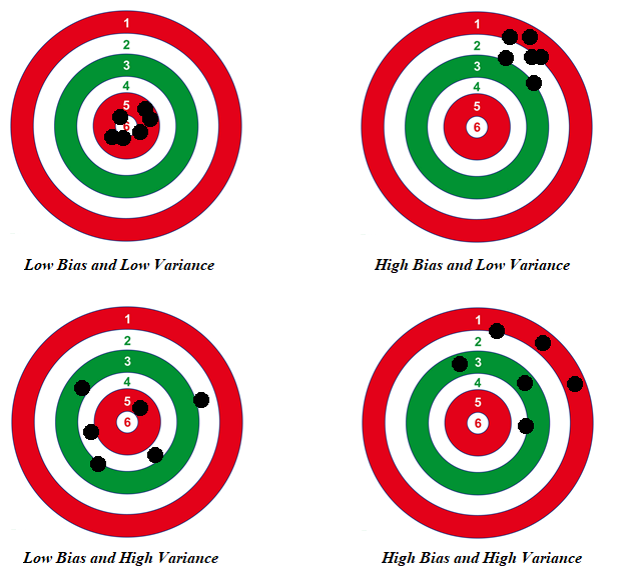
\includegraphics[scale=.45]{../05-pictures/lesson-2-2_pic_14.png}  
\end{center}
\end{frame}
%..................................................................
\begin{frame}{Bias and Variance}
\begin{tcolorbox}
Unfortunately, we often find that there is a trade-off between bias and variance. As one is reduced, the other is increased. This is the matter of over- and under-fitting.
\end{tcolorbox}
\begin{center}
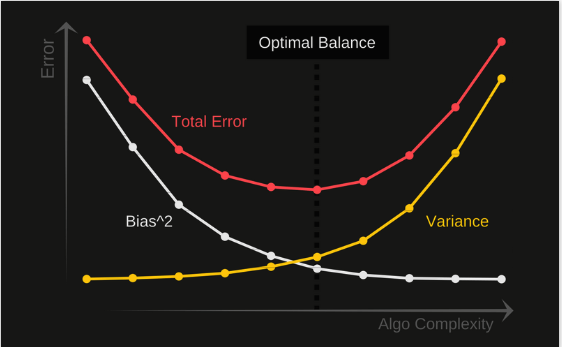
\includegraphics[scale=.4]{../05-pictures/lesson-2-2_pic_15.png} 
\end{center}
\end{frame}
%__________________________________________________________________________
%
\subsection[subsection]{Regularization}
%__________________________________________________________________________
%
\begin{frame}{Regularization}
	\begin{itemize}
		\item Linear regression can over-fit, particularly when there are a large number of correlated features.
		\item Results for validation set may not then be as good as for training set
		\item Regularization is a way of avoiding overfitting and reducing the number of features. Alternatives:
		\item Ridge 
		\item Lasso
		\item Elastic net
		\item We must first scale feature values
	\end{itemize}
\end{frame}
%..................................................................
\begin{frame}{Ridge regression (analytic solution)}
	\begin{itemize}
\item Ridge regression is a regularization technique where we change the function that is to be minimize;	
		\item Reduce magnitude of regression coefficients by choosing a parameter $\lambda$ and minimizing
		\begin{equation}
		\frac{1}{2N} \sum\limits_{n=1}^N \left[h_\theta \left( x^{(n)} \right) - y ^{(n)}\right]^2	+ \highlight{\lambda \sum\limits_{n=1}^N b_i^2}
		\end{equation}
		\item This change has the effect of encouraging the model to keep the weights $b_j$ as small as possibile;
		\item The Ridge regression should only be used for determining model parameters using the training set. Once the model parameters have been determined the penalty term should be removed for prediction;
		\item What happens as $\lambda$ increases?
	\end{itemize}
\end{frame}
%..................................................................
\begin{frame}{Lasso Regression (must use gradient descent)}
	\begin{itemize}
	\item Lasso is short for \textit{Least Absolute Shrinkage and Selection Operator};
		\item Similar to ridge regression except we minimize
		\begin{equation}
		\frac{1}{2N} \sum\limits_{n=1}^N \left[h_\theta \left( x^{(n)} \right) - y ^{(n)}\right]^2 + \highlight{\lambda \sum\limits_{n=1}^N \vert b_n \vert}
		\end{equation}
		\item This function cannot be minimized analytically and so a variation on the gradient descent algorithm must be used;
		\item Lasso regression also has the effect of simplifying the model. It does this by setting the weights of unimportant features to zero. When there are a large number of features, Lasso can identify a relatively small subset of the features that form a good predictive model.
	\end{itemize}
\end{frame}
%..................................................................
\begin{frame}{Ridge and Lasso Regression Compared}
\begin{center}
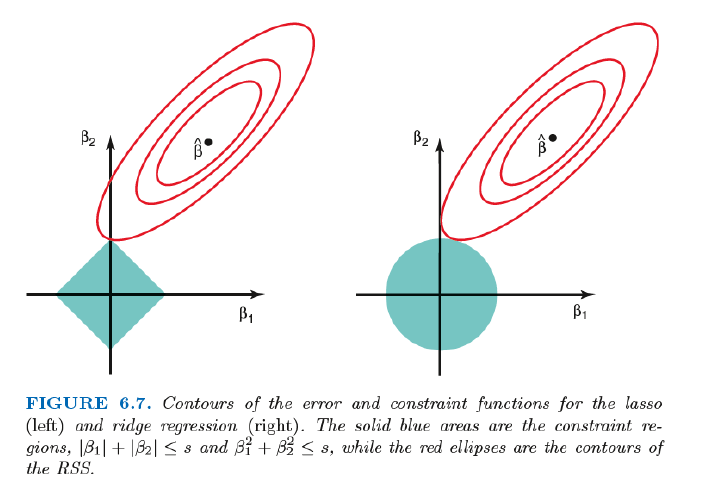
\includegraphics[scale=.55]{../05-pictures/lesson-2-2_pic_16.png} 
\end{center}
\end{frame}
%..................................................................
\begin{frame}{Elastic Net Regression (must use gradient descent)}
	\begin{itemize}
		\item Middle ground between Ridge and Lasso
		\item Minimize
		\begin{equation}
		\frac{1}{2N} \sum\limits_{n=1}^N \left[h_\theta \left( x^{(n)} \right) - y ^{(n)}\right]^2 + \highlight{\lambda_1 \sum\limits_{n=1}^N b_n^2 + \lambda_2 \sum\limits_{n=1}^N \vert b_n \vert}
		\end{equation}
		\item In Lasso some weights are reduced to zero but others may be quite large. In Ridge, weights are small in magnitude but they are not reduced to zero. The idea underlying Elastic Net is that we may be able to get the best of both by making some weights zero while reducing the magnitude of the others.
	\end{itemize}
\end{frame}
%..................................................................
\begin{frame}{Salary Vs Age Example: The Effect of Regularization}
	\begin{center}
	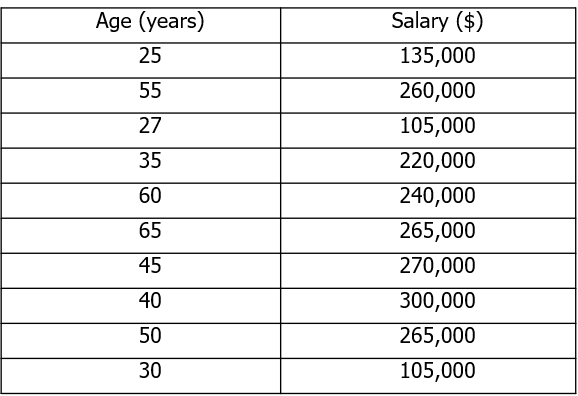
\includegraphics[scale=.4]{../05-pictures/lesson-2-2_pic_17.png}
	\end{center}
We apply regularization to the model:
\begin{equation}
Y = a + b_1X + b_2X^2 + b_3X^3 + b_4X^4 + b_5 X^5
\end{equation}
where $Y$ is salary and $X$ is age.
\end{frame}
%..................................................................
\begin{frame}{Salary Vs Age Example: The Effect of Regularization}

Data with Z-score scaling
	\begin{center}
	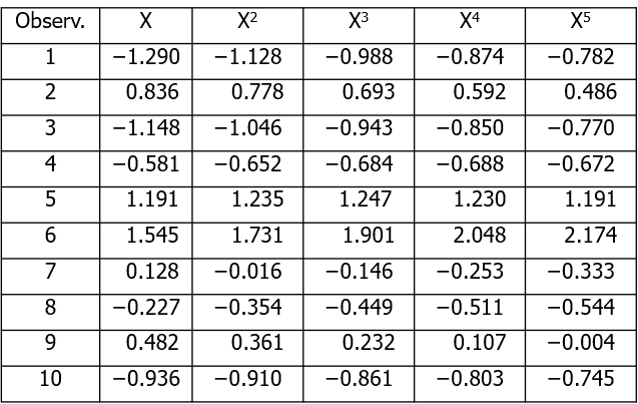
\includegraphics[scale=.6]{../05-pictures/lesson-2-2_pic_18.png}
	\end{center}
\end{frame}
%..................................................................
\begin{frame}{Salary Vs Age Example: The Effect of Regularization}
Ridge Results, $\lambda=0.02$ is similar to quadratic model
	\begin{center}
	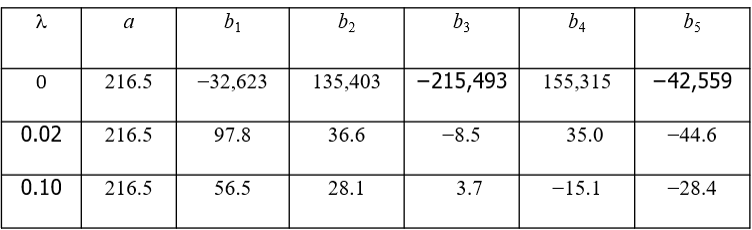
\includegraphics[scale=.55]{../05-pictures/lesson-2-2_pic_19.png}
	\end{center}
\end{frame}
%..................................................................
\begin{frame}{Salary Vs Age Example: The Effect of Regularization}

Lasso Results, $\lambda=1$ is similar to the quadratic model

	\begin{center}
	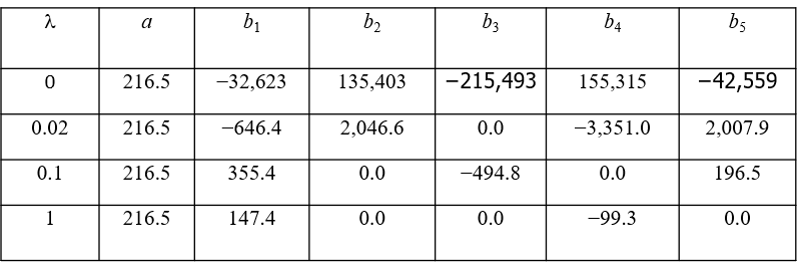
\includegraphics[scale=.5]{../05-pictures/lesson-2-2_pic_20.png}
	\end{center}
\end{frame}
%..................................................................
\begin{frame}{Let's code ...}
%\begin{center}
%\includegraphics[scale=.8]{../05-pictures/exercise.jpg} 
%\end{center}
\end{frame}
%===================================================================================================
\end{document}

